%%%%%%%%%%% ******  AUTOMATED PLANNING ******* %%%%%%%%%%%%%
\section{Introduction}
\begin{center}
\textit{``Planning is an important component of rational behaviour." }\\ \cite{ghallab2004automated}
\end{center}

% \begin{center}
% \textit{``A goal without a plan is just a wish."}\\
% - Antoine de Saint-Exup\'{e}ry
% \end{center}

% Introduction/Definition
Automated planning, also known as AI planning, is an area in A.I. that studies the deliberation process of choosing and organising actions to achieve a goal. 
Humans automatically anticipate the outcome of their actions, even if they are not fully aware of it. 
Automated planning techniques are used to create information processing tools that efficiently reproduce human reasoning and behaviour. 
In particular, it can be used to model a robot's skills and strategies, when operating in diverse environments, without the need for expensive hand-coding.

The focus in automated planning lies within the development of {domain-independent} planning systems, called \textit{planners}.
These planners consist of search algorithms, which are not problem-specific, hence generate solutions to problems, no matter what the input. 
Given a set of actions, a description of the state of the world, and some goal state, the planner generates an ordered sequence of actions, which guarantees the transition from the initial state to the goal state. 
Actions are defined with \textit{preconditions}, \ie conditions on the state of the world in order to execute the action, and \textit{effects}, \ie changes in the state of the world after the action execution.
Planning can be considered the process of choosing appropriate actions to bring the state of the world to a target state.
In the following section we will present the main definitions used in classical planning.
%The planner produces an ordered sequence of actions, known as a \textit{plan}, which guarantees the transition from the initial state to the goal state.
%For instance, there exist different types of planning:
%\begin{itemize}
%    \item Classical planning
%    \item Optimisation: minimise or maximise a given cost function
%    \item Temporal planning: actions have a certain duration, to address concurrency, synchronisation, time dependent effects
%    \item Planning with preferences: prefer hard goals over soft goals
%    \item Conditional planning: actions can perform observations, plan contains branches
%\end{itemize}

\section{Classical planning}\label{subsec:Classical planning problem}
In classical planning, world dynamics are modelled as state transition systems. 
We will start by providing some definitions of general concepts used in this thesis that have been derived from \cite{ghallab2004automated}.


\begin{definition}
A \textit{state transition system} is a triple $\Sigma = (S, A, \gamma)$ such that:
\begin{itemize}
\item $S=\{s_1, s_2, \dots \}$ is a finite set of states,
\item $A=\{a_1, a_2, \dots \}$ is a set of actions,
%\item $c : A \rightarrow \mathbb{R}^{+}$ is a cost function,
\item $\gamma : S \times A \rightarrow S$ is a state transition function.
\end{itemize}
\end{definition}

A state transition system $\Sigma$ can be represented as a directed graph whose nodes are states of $S$ and arcs are actions of $A$. 
Applying an action $a$ to state $s$ produces a new state $s'= \gamma(s,a)$ that is represented as an arc from $s$ to $s'$, referred to as a  \textit{state transition}.
%with a cost $c(a)$
$\Sigma$ is deterministic if for all states $s$ and actions $a$ and the transition function $\gamma(a, s)$ produces a unique state $s'$. 
%$\Sigma$ has a unit cost if, for all $a \in A$, $c(a) = 1$. 


%\begin{figure}[t]
%	\centering
%	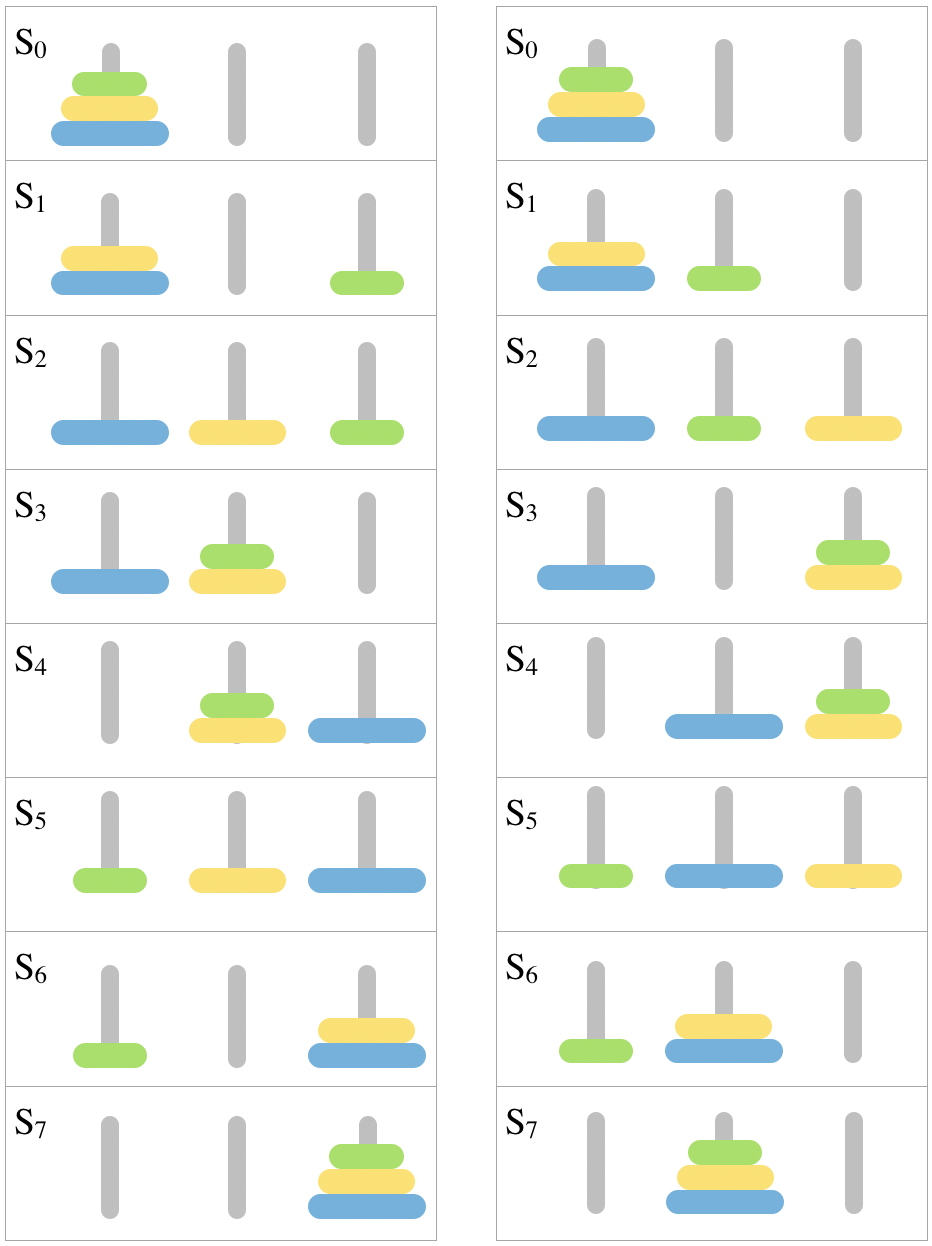
\includegraphics[width=0.7\textwidth]{figures/toh-solutions}
%	\caption{Examples of plans to the Tower of Hanoi problem, starting from an initial state $S_0$ but moving towards different goal states, where the set of actions $A$ consists of moving a disc from one peg to another.}
%	\label{fig:toh-solutions}
%\end{figure}

%\subsubsection{Classical Planning Representations}

%Classical planning problems can be represented in three different ways, each of them being equivalent in expressive power: \cite{ghallab2004automated}

%\begin{itemize}
%\item Set-theoretic representation: each state of the world is a set of propositions, each action is a syntactic expression specifying which propositions belong to the state in order for the action to be applicable (\eg \texttt{ontable-red, ontable-blue, on-red-blue, holding-red, holding-blue, stack-red-blue})
%\item Classical representation: states and actions are like the ones in set-theoretic representations except that first-order literals and logical connectives are used instead of propositions (\eg \texttt{ontable(x), on(x,y), holding(x), stack(x,y)} )
%\item State-variable representation: each state is represented by a tuple of values of n state variables \{\texttt{red, blue,\dots, table, 1, 0, nil}\} (\eg \texttt{pos(x) = table, pos(x) = y, holding = x, stack(x: block, y: block)})
%\end{itemize}

%\noindent The set-theoretic representation can take up much more space than the classical representation. The state-variable representation is less natural for logicians but useful for non-classical planning problems to handle numbers, function and time. The classical representation is the most popular choice for restricted state-transition systems \cite{ghallab2004automated}.

Logical representations are one of the most commonly used representations for classical planning problems. 
Each state of the world $s$ is represented by a set of logical propositions $p$, denoting facts of the world that are \textit{true} in the state $s$. 
If $p$ is not in the state $s$, it is considered to be \textit{false}.

\textit{Planning operators} change the state of the world by modifying the truth values of the propositions. 
An operator is defined by a set of propositions, which have to be true in a state in order to apply the action (\textit{preconditions}), and a set of propositions, which will be true or false after the application of the action (\textit{effects}).

\begin{definition}
A \textit{planning operator} $o$ is a tuple $o = (\text{name}(o), \text{precond}(o),$ $\text{effect}(o))$, whose elements are as follows:
\begin{itemize}
	\item $\text{name}(o)$ is the {\em name} of the operator,
	\item $\text{precond}(o)$ is a set of literals that must be true to apply the operator $o$,
	\item $\text{effect}(o)^{-}$ is a set of literals that are false after the application of the operator $o$,
	\item $\text{effect}(o)^{+}$ is a set of literals that are true after the application of the operator $o$,
\end{itemize}
\end{definition}
where $\text{effect}(a) = \text{effect}(a)^{-} \cup \text{effect}(a)^{+}$ and $\text{effect}^{-}(a) \cap \text{effect}^{+}(a) = \emptyset$. 
An operator is applied to a set of parameters that are associated with a \textit{type}.
For example, a general type could be \textit{OBJECT} or \textit{POSITION}.
Some planning problems include type hierarchies with a general type (\eg OBJECT) that consists of subtypes (\eg BASE and CUBE).

\begin{definition}\label{def:action}
	An \textit{action} is any ground instance of an operator. 
	If $a$ is an action and $s$ is a state such that $\text{precond}(a)$ are true in $s$, then $a$ is {\em applicable} to $s$ and the result of applying action $a$ to state $s$ is the state $s'$:  
	\begin{equation}\label{eq:statetrans}
		s' = \gamma(s, a) = (s - \text{effects}^{-}(a)) \cup \text{effects}^{+}(a),
	\end{equation}
	
\end{definition}

%For each $a \in A$, $\text{precond}(a)$ and $\text{effect}(a)$ are subsets of $S$ and . 
We consider an operator as as a \textit{generalised} action.

\begin{definition}
A \textit{planning domain} is a state transition system $\Sigma = (S, A, \gamma)$, with the state transition function stated as in Eq. \ref{eq:statetrans}.
\end{definition}

\begin{definition}
A \textit{planning problem} is a triplet $(\Sigma, s_0, g)$ where:
\begin{itemize}
%	\item $P$ is a finite set of propositions,
%	\item $A$ is a finite set of actions,% where for each $a \in A$, $\text{precond}(a), \text{effect}(a) \subset P$
	%\item $c : A \rightarrow \mathbb{R}^{+}$ is a cost function,
	\item $s_0 \subseteq S$ is the initial state of the world,
	\item $g$ is a set of goal propositions that belong to the goal states to achieve.
\end{itemize}
\end{definition}

\begin{definition}
	A \textit{plan} is any sequence of $k$ actions $\pi = \langle a_1,\cdots, a_k\rangle$, where $k\geq 0$. 
\end{definition}
The state produced by applying $\pi$ to a state $s$ is the state obtained by applying each action of $\pi$ sequentially. 
We can denote this by extending the state transition function to plans as follows:
\[\gamma(s,\pi)=\left\{
\begin{array}{ll}
s, &\mbox{if $|\pi|=0$} \\
\gamma(\gamma(s,a_1),\langle a_2,\cdots, a_k\rangle ), &\mbox{if $|\pi|>0$ and $a_1$ is applicable to $s$} \\
\mbox{undefined}, &\mbox{otherwise.}
\end{array}
\right.
\]
A state $s_n$ is reachable from a state $s_0$, if there exists a plan $\pi$ such that $s_{n} = \gamma(s_0, \pi)$.
When a full specification (planning domain and problem) are provided to the planner, it generates a plan to achieve the specified goals using the available actions.
Thus, a plan is a \textit{solution} to a planning problem if it guarantees the transition from the initial states $s_0$ to the goal states, \ie $g \subseteq \gamma (s_0,\pi)$. 

%The {\em state space} of a planning problem $(P, A, I, G)$ in the logical representation is a state transition system $(S, A, \gamma)$, where $S\subseteq 2^{P}$ is a subset of states defined on $P$.\\


%Once this specification is provided to the planner, the planning process is a mean-ends reasoning, deciding how to achieve goals given the means of available actions. The hardness of the mean-ends planning process is high (NP-hard), as it entails non-deterministic decisions on selecting objects, committing actions on objects, sorting out actions, as well as backtracking from dead-end decisions in combinatorial search spaces.

When actions are triggered, they change the state of the world according to their effects and are not necessarily reversible. 
In other words, actions are not combinable in any order and have precedence constraints. 
For example, with the Tower of Hanoi problem, the two last actions consist of stacking the second smallest disk and then the smallest disk on the peg. 
Reversing the order will result in a violation of the rule that larger disks cannot be stacked onto smaller ones. Thus, plans need to be performed in the correct order to achieve the a goal.

Furthermore, the progression towards the goal is not always monotone, as actions can also have negative side effects. 
Consider again the Tower of Hanoi problem, where the disks need to be stacked in ascending order (smallest at the top) on the right-most peg. 
Our goal state is to have \textit{``disk$_{n}$ is on top of disk$_{n+1}$"} and \textit{``disk$_{n+1}$ is on the table"} for a problem with $n>0$ disks. 
If in the initial state the disks are stacked in ascending order on the left peg, then moving the top-most disk$_1$ to any other peg will delete the fact \textit{``disk$_1$ is on top of disk$_2$"}, and will have to be added again later to fulfill the goal (\fig{fig:toh-solutions}).


%\subsection{STRIPS}\label{subsec:STRIPS}
%In STRIPS a closed-world assumption is used, \ie any conditions that are not mentioned in a state are assumed to be false.


%%%%%%%%%%%%%%% *************PDDL************* %%%%%%%%%%%%%%%%%
\section{Planning Domain Definition Language (PDDL)}\label{subsec:PDDL}
Originally developed by \cite{mcdermott1998pddl} and Planning Competition Committee, the Planning Domain Definition Language (PDDL) has become the standard encoding language for classical planning tasks. It supports several syntactic features including conditional effects, specification of safety constraints and hierarchical actions composed of subactions and subgoals. PDDL expresses the ``physics'' of a domain, \ie the available predicates, the possible actions and their effects.
The PDDL planning domain can be used to formalise the configuration of available resources together with the intended goal to eventually find a solution using PDDL planners  (\cite{huckaby2013planning}). 
%Table \ref{tab:Domain examples} shows a list of standard planning domains. 
%
%\begin{table}[h]
%\begin{center}
%\begin{tabular}{l|l|l}
%Domain & Types & Action models \\ \hline
%Blocks world & block & pick-up, put-down, stack, unstack \\
%Gripper & room, ball, gripper & pick, drop, move \\
%Tetris & L-block, S-block, I-block, T-block, O-block & pick-up, put-down, move, rotate\\
%\end{tabular}
%\end{center}
%\label{tab:Domain examples}
%\caption{Examples of possible domains with action models to be learned}
%\end{table}

\subsection{Planning domain description}\label{subsec:Planning domain description}
A PDDL planning domain consists of objects and their types, predicates describing the state of an object, and actions. 
Consider a planning domain that describes a simple pick-and-place scenario with three types of objects (BASE, CUBE, ROOF).
%manufacturing environment on an assembly line, with objects on the table and an arm with a gripper for manipulating them.
The head of a domain description is given as follows:
% Head of the domain description
\begin{verbatim}
(define (domain iRoPro)
 (:requirements :typing :strips)
 (:types 
  element 
  position - element 
  object - element 
  cube - object 
  base - object 
  roof - object )
 (:predicates
  (clear ?obj - element)
  (thin ?obj - element)
  (flat ?obj - element)
  (on ?obj2 - object ?obj1 - element)
  (stackable ?o - object ?e - element) 
)
\end{verbatim}

A domain description always starts with the declaration of its name, preceded by the keyword \texttt{:domain}. 
%Then, the requirements of the domain are defined, . 
The requirements (identified by the keyword \texttt{:requirements}) allow to characterise the expressiveness of the domain description. 
For instance, in the domain description above, the requirements specify that action descriptions can use typed terms. In other cases, preconditions with equality terms, and effects, with conditional and universal quantifier terms, can also be specified. 

All domains define a few primitive types from which it is possible to derive all the types necessary for the domain description. 
In the above example domain, the types \texttt{base, cube} and \texttt{roof} are derived from the type \texttt{object}. 
The type descriptions are identified by the keyword \texttt{:types}. 
%The keyword \texttt{:constants} defines the values that remain unchanged and that can be referenced directly.

The predicates, identified by the keyword \texttt{:predicates}, specify what facts (about objects in the world) can be used in the preconditions and effects of the operators.
Predicates can have arguments of specified types. 
An argument term starts with a question mark `\texttt{?}'. 
For instance, \texttt{(on ?o - object ?e - element)} expresses that a variable \texttt{?o}, whose type is \texttt{object}, is positioned on an element \texttt{?e}.

The above planning domain is comprised of the following predicates, which can be seen as logical symbols:

\begin{table}[h]
\begin{center}
\begin{tabular}{l|l}
Predicate in PDDL & Description in English\\ \hline
(clear ?obj - element) & an element has nothing on top of it \\
(thin ?obj - object) & an object is thin\\
(flat ?obj - element) & an element has a flat top \\
(on ?obj2 - object ?obj1 - element)& an object is on an element\\
(stackable ?o - object ?e - element) & an object can be placed on an element\\
%\texttt{at-gripper ?g - gripper ?l - location} & The gripper \texttt{?g} is at position \texttt{?l}.\\
%\texttt{at ?p - product ?l - location} & The product \texttt{?p} is at location \texttt{?l}.\\
%\texttt{free ?g - gripper} & The gripper \texttt{?g} is free.\\
%\texttt{carry ?p - product ?g - gripper} & The gripper \texttt{?g} is holding product \texttt{?p}.\\
%\texttt{empty ?l - location} & The location \texttt{?l} is empty.\\
\end{tabular}
\end{center}
\label{tab:predicates}
\caption{Predicates for the \texttt{} domain}
\end{table}%


In a domain description, operators, \ie first-order actions, specify the different ways to perform changes to the world state. 
In general, an action model consists of the following (see \fig{fig:action model}):
\begin{itemize}
	\item \texttt{:parameters} -- variables on which the action model operates,
	\item \texttt{:precondition} -- conditions that must be satisfied before the action can be executed; if none are specified, the action is always executable,
	\item \texttt{:effect} -- changes in the world state imposed by the action.
\end{itemize}

\begin{figure}[h]
	\centering
	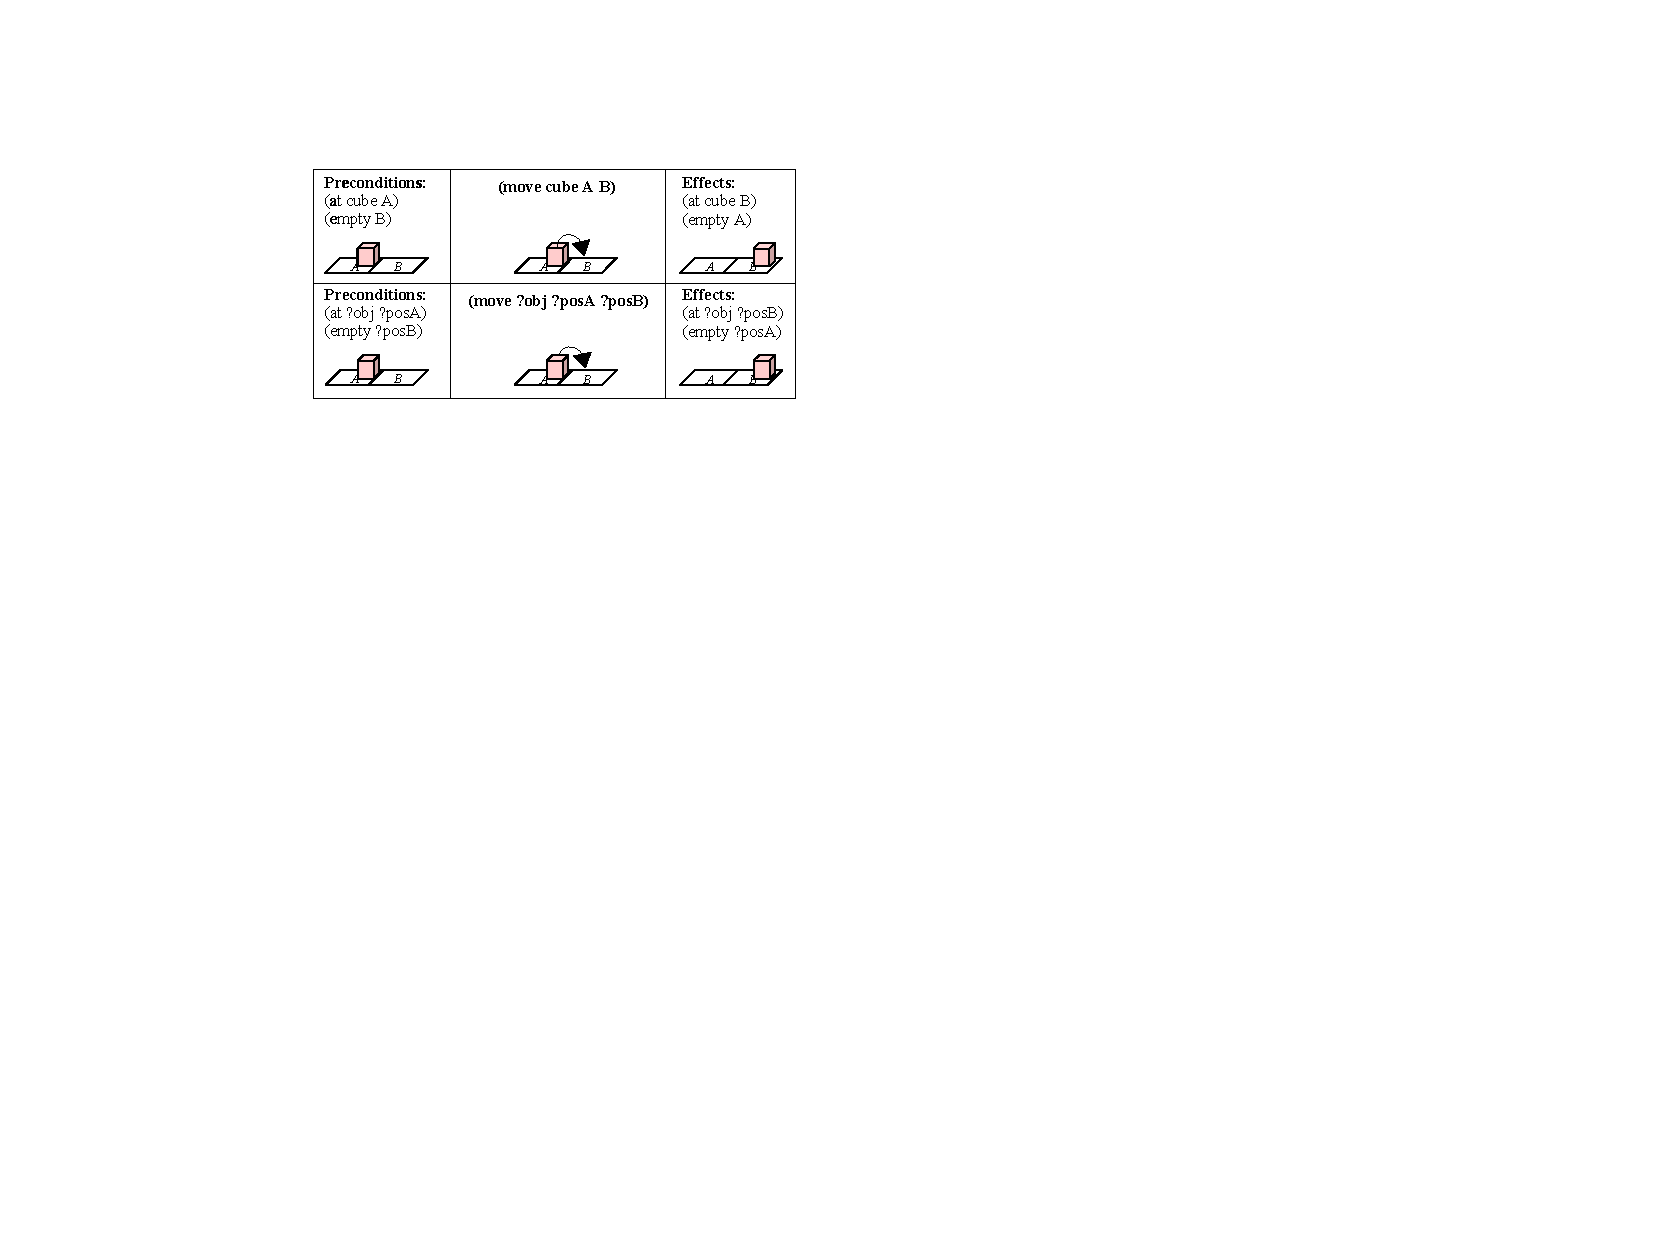
\includegraphics[width=0.8\textwidth]{figures/schema-logic}
	\caption{Action model representation of a move action in terms of preconditions and effects: demonstrated action model for a cube (top), and generalised action model for any object, variables are prefixed with `?' (bottom).}
	\label{fig:action model}
\end{figure}

Consider a simple move action, which consists of grasping an object with the gripper and results in lifting it off the table.
\begin{verbatim}
(:action move
 :parameters (?obj - object ?A - position ?B - position)
 :precondition (and (on ?obj ?A) (clear ?B)
                       not(on ?obj ?B) not(clear ?A))
 :effect (and (on ?obj ?B) (clear ?A)
                       not(on ?obj ?A) not(clear ?B))
\end{verbatim}

This action means that an object (\texttt{?obj}) can be picked up, if both the object and the target position (\texttt{?B}) are clear.
%if both the gripper \texttt{?g} and the product are at the location \texttt{?l} and the gripper is free (preconditions). 
After the \texttt{move} action execution, the effects express that the object is no longer at initial position \texttt{?A} but on \texttt{?B} and that \texttt{?A} is clear, but \texttt{?B} is not.
%gripper \texttt{?g} is currently carrying the product \texttt{?p}, that it is not free anymore and that the product is no longer placed at location \texttt{?l}.


%The \texttt{PRODUCTION} domain consists of the three actions: \texttt{pick, drop} and \texttt{move}. Similar to the \texttt{pick} action, \texttt{drop} can be specified as follows:
%\begin{verbatim}
%   (:action drop
%       :parameters  (?p - product ?l - location ?g - gripper)
%       :precondition  (and  (carry ?p ?g) (at-gripper ?g ?l) (empty ?l))
%       :effect (and (at ?p ?l)
%                    not(empty ?l)
%                    (free ?g))))
%\end{verbatim}
%In this action, product \texttt{?p} is dropped at a location \texttt{?l}. The preconditions assert that product \texttt{?p} has to be carried by the gripper \texttt{?g} and that the gripper \texttt{?g} is at the location \texttt{?l}, which is empty.  The effects mean that after the action execution, the product \texttt{?p} occupies location \texttt{?l} and that the gripper \texttt{?g} is free. \\
%Consider the last action in our domain:
%\begin{verbatim}
%   (:action move
%       :parameters  (?g - gripper ?from ?to - location)
%       :precondition (at-gripper ?g ?from)
%       :effect (and  (at-gripper ?g ?to)
%                     (not (at-gripper ?g ?from))))
%\end{verbatim}
%This specifies that the gripper \texttt{?g} moves from a starting position \texttt{?from} to a target position \texttt{?to}, if the gripper is initially at starting position \texttt{?from}. The predicates \texttt{(at-gripper ?g ?to)} and \texttt{(not (at-gripper ?g ?from))} in the effect description ensure that the gripper is not at two positions at the same time.
%\begin{itemize}
%\item Example state of the art: (example action sequence)
 % \item{   Manufacturing tasks require extra overhead to {reprogram the robot} when the process of the task changes.  }
  %\item{   A key issue in PbD is to {design a generic system} to teach skills that can be used in different situations.  }
  %\item{   Current implementations include an {intermediate manual step to construct action sequences} to arrive to a goal state.  }
%  \end{itemize}


\subsection{Planning Problem Description}\label{subsec:PPDescription}
%In manufacturing domains, there exist installation procedures for various devices that need to be strictly followed. 
%It can happen that assembly parts need to be moved around in the work place. 
%Consider a planning problem for the above domain:
A planning problem consists of an initial state and a goal state and can only be solved using existing actions in the domain.
For example, the problem of swapping two objects obj1, obj2 on A and B respectively with C unoccupied, can be defined as:

\begin{verbatim}
(define (problem swap)
  (:domain iRoPro)
  (:objects posA posB posC - position
                obj1 obj2 - base)
  (:init (on obj1 posA)(on obj2 posB) (clear posC))
  (:goal (on obj1 posB) (on obj2 posA) )
)
\end{verbatim}
%(define (problem PERMUTATION)
%(:domain PRODUCTION)
%(:requirements :typing)
%(:objects zoneA zoneB - zone
%table - table
%engine - metal
%hood - metal)
%(:init (at-gripper zoneA)
%(free right)
%(at engine zoneB)
%(at hood zoneA))
%(:goal (at engine zoneA)
%(at hood zoneB)))

The planning problem is defined using a name and by specifying the domain it operates in.
It then lists all objects of the world and their initial states (\fig{fig:planning problem}ab). 
This world is composed of three positions, \texttt{A}, \texttt{B} and \texttt{C}, and two objects, \texttt{obj1} and \texttt{obj2}, which are both of type \texttt{base}. 
The initial state of the world is that two \texttt{obj1} and \texttt{obj2} are on \texttt{A} and \texttt{B} respectively with \texttt{C} unoccupied.
%The engine needs to be installed before the hood, therefore the engine needs to be placed in \texttt{A} and the hood needs to be in \texttt{B}. As devices on assembly lines arrive arbitrarily, depending on the completion time of the previous task, it is possible that they arrive in the reversed order. 
Given only one gripper, the goal is to find a plan to move \texttt{obj1} from \texttt{A} to \texttt{B} and \texttt{obj2} from \texttt{B} to \texttt{C} (\fig{fig:planning problem}d). 
The planner would generate the following action sequence (\fig{fig:planning problem}c):
\begin{verbatim}
1. move(obj1, A, C)
2. move(obj2, B, A)
3. move(obj1, C, B)
\end{verbatim}

\begin{figure}[h]
	\centering
	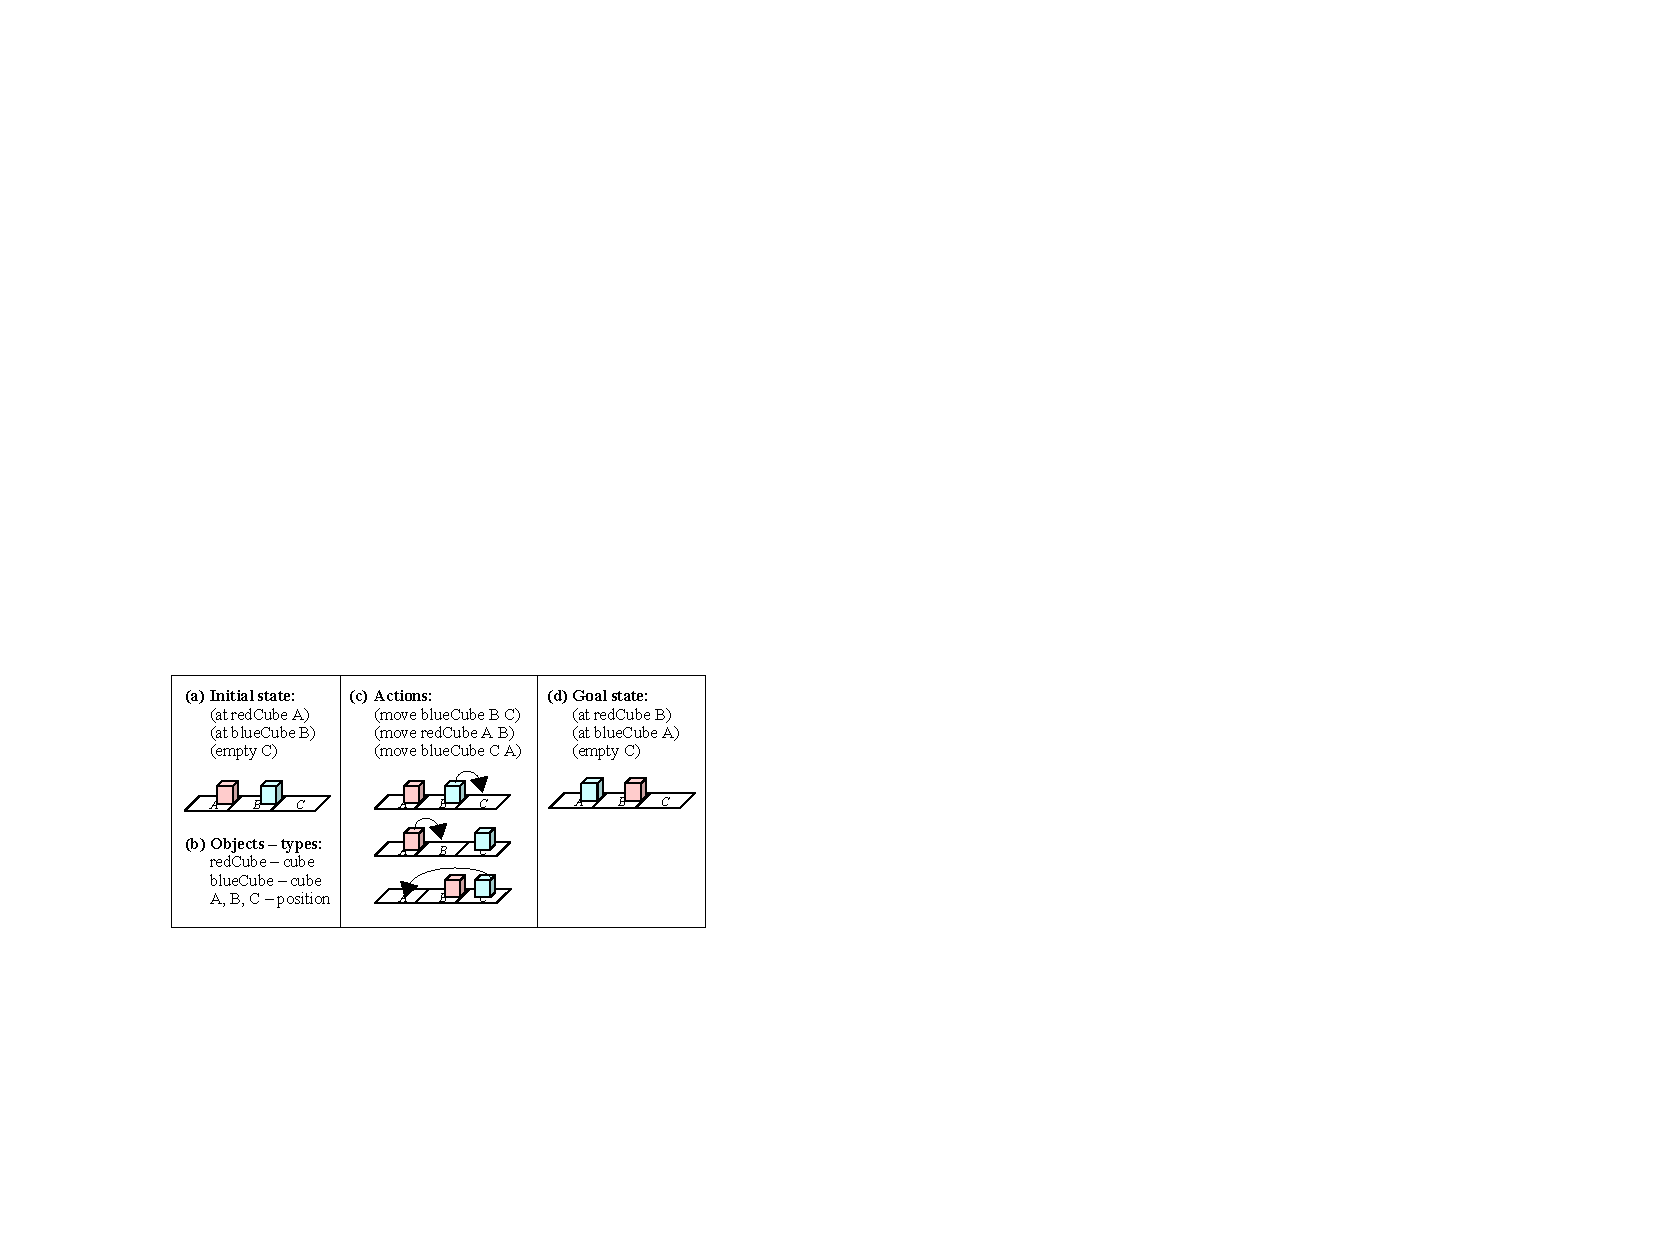
\includegraphics[width=0.8\textwidth]{figures/planning-permutation}
	\caption{Definition of a planning problem: (a) properties describing the initial world state (b) object names and their types (c) instantiated actions (d) properties describing the goal state}
	\label{fig:planning problem}
\end{figure}

Another planning problem in this domain could include multiple objects of different types which need to be stacked in a given order, such as the Tower of Hanoi problem.
As we can define an infinite number of objects in our planning domain, there exist an infinite number of planning problems that can be defined and solved. 
PDDL provides a means to model any real-world environment in the form of a planning domain. 


\subsection{PDDL evolution and extensions}\label{subsec:PDDL evolution}

Ever since the first version of \textsc{Pddl} 1.2 (\cite{mcdermott1998pddl}) was introduced as the official language of the 1st \textsc{Ipc} (International Planning Competition), there have been several new versions and extensions.
Succeeding versions that allow the representation of real-world problems had a particular influence on the adaptation of planners with robots in cobotic environments. 
In 2002, \textsc{Pddl} 2.1 introduced functions to express numerical objects, durative actions and plan-metrics for assessing plan quality.
An extension called \textsc{Mapl} (Multi-Agent Planning Language), introduced finite domain state-variables, actions with duration determined in runtime, and explicit plan synchronisation obtained through speech acts and communications among agents. 
The newly introduced functionalities are particularly useful for cobotic environments to incorporate actions of varying durations into the planning system, or to allow multi-agent planning for several robots to collaborate in the same environment.
In the following years \textsc{Ppddl} (Probabilistic \textsc{Pddl})(\cite{younes:04a}) was proposed, extending \textsc{Pddl} 2.1 with probabilistic effects and introducing partial observability. 
This extension opened up the possibility to integrate statistical models into the planning system and improved the robot's learning capabilities and performance in uncertain situations. 
Cobots can benefit from this as they are often faced with uncertain situations when working with different human operators, who have varying behaviours.

\subsection{Planners}\label{subsec:Planners}
Automated planners have found increasing applications in various areas from aeronautics and space to agricultural and industrial domains (\cite{aarup1992optimum}). 
The majority of planning procedures are search procedures, where the difference lies in the search spaces.
We conclude this section by introducing the most commonly known techniques for classical planning (Table \ref{tab:planningapproaches}):
state-space planning, plan-space planning, and planning graphs. 
We refer the reader to \cite{nau2007current} who provides a more detailed overview of the techniques with accompanying illustrations.

%Nearly all planning procedures are search procedures - Different planning procedures have different search spaces
% 1. state space planners: 
% Each node represents a state of the world »A plan is a path through the space
The simplest planners are state-space planners (\cite{ghallab2004automated}), which rely on search algorithms in which the search space is a subset of the state space. 
Each node corresponds to a state of the world, each arc represents a state transition, \ie an action, and a plan is a path from the initial state to a goal state in the search space. 
An extended version of the planner is the Heuristics Search Planner (\cite{bonet:01}), which includes several basic search algorithms like breadth-first search, best-first search (\eg A*) and iterative deepening search. 
The Fast Forward planning system (\cite{hoffmann2001ff}) is based on the HSP, but managed to outperform it, due to modifications aimed to avoid getting trapped in local minima. % (\cite{hoffmann2000heuristic}): 
%It includes a variation of the hill-climbing search, called the \textit{enforced hill climbing}, and a heuristic called \textit{helpful actions}. 
Finally, Fast Downward (\cite{helmert:06a}) is a state-space planner based on a finite domain representation, with a greedy best-first search as its main search procedure. 
% Problem with state-space search : we may try many different orderings of the same actions before realizing there is no solution -> Least-commitment strategy: don’t commit to orderings, instantiations, etc., until necessary
The problem with state-space search is that it commits to plan step orderings, meaning that many different orderings of the same actions are considered even if none of them lead to a solution.

% 2. plan space planners : Backward search from the goal 
% Each node is a set of partially-instantiated operators, plus some constraints »Impose more and more constraints, until we get a plan
A second category known as plan-space planners (\cite{chapman1987planning,mcallester1991systematic}) handle goal orderings in an optimal way and are generally considered more efficient. 
%The adaptation method is based on a constraint-posting technique of Chapman [1987] and its laterrefinement [McAllester and Rosenblitt 1991]. The fitted plan to be adapted constitutes a node in thesearch space and the search starts from there instead of traversing the space of partial-order plans inbreadth-first manner starting from the root, as SNLP does
For such partial-order planners each node is a set of partially instantiated-operators with constraints (\eg temporal constraints for the application of an action).
The idea is to perform a backward search from the goal and impose an increasing number of constraints until a complete plan has been found.

%
% 3. planning-graph techniques
Another category are planning-graph planners, first introduced in the Graphplan (\cite{blum:97}).
The idea is to encode the search space in a structure called the \textit{planning graph} that is much smaller than the state transition graph and contains information about possibly reachable states.
%It uses a backward search by  and replaces the goal with preconditions.
The true set of reachable states can be quickly estimated by eliminating many impossible ones in the search process.
A plan is then extracted from the planning graph.
%It considers the union of sets of propositions of several reachable states rather than individual states.  
% other planners
Other graph-based planners include SATPlan (\cite{kautz:06,kautz:99}), that uses a \textsc{Sat} solver, and the GP-CSP (\cite{do:01}) that uses a \textsc{CSP} solver.

\begin{table}[h]
	\centering
	\begin{center}
		\begin{tabular}{@{\hskip0pt}l@{\hskip2.5pt}l@{\hskip1.5pt}l@{\hskip1.5pt}} \hline
			\textbf{Approach} & \textbf{Generated Plan} & \textbf{Planning Systems}\\ \hline
			State-space & sequence of actions &
			\begin{tabular}{l}
				HSP (\cite{bonet:01})\\
				\textsc{Ff} (\cite{hoffmann2001ff})\\
				\textsc{Fd} (\cite{helmert:06a}) \\
				\textsc{Lama} (\cite{richter2010lama}) \\
			\end{tabular}\\ \hline
			Plan-space & partially ordered set of actions &  
			\begin{tabular}{l}
				TWEAK (\cite{chapman1987planning})\\
				SNLP (\cite{mcallester1991systematic})\\
				UCPOP (\cite{penberthy1992ucpop})\\
				O-Plan (\cite{tate1994plan2})\\
				FAPE (\cite{dvo2014plan})\\
			\end{tabular}\\ \hline
			Planning graph & sequence of sets of parallel actions &
			\begin{tabular}{l}
				Graphplan (\cite{blum:97})\\
				\textsc{Stan} (\cite{long1999efficient})\\
				CSP (\cite{lopez2003generalizing})\\
				weighted CSP (\cite{cooper2011weighted})\\
				SATPlan (\cite{rintanen2014madagascar})\\
			\end{tabular}\\ \hline
%			Other & sequence of sets of parallel actions &
%			\begin{tabular}{l}
%				\textsc{Stan} (\cite{long1999efficient})\\
%				Blackbox (\cite{kautz:99})  \\
%			\end{tabular}\\ \hline
		\end{tabular}
	\end{center}
	\caption{Main automated planning approaches and systems}
	\label{tab:planningapproaches}
\end{table}

There exist other planning techniques such as model checking (\cite{triantafillou2015unifying}) or Markov Decision Process (\cite{kolobov2012planning}) but there is no single planning strategy or domain-independent search heuristic that is universally better than others.

The main open-source planning toolkits are the Lightweight Automated Planning ToolKit (\cite{lapkt}), based on Fast Downward and Fast Forward, and PDDL4J, a Planning Domain Description Library for Java cross-platform developers (\cite{pellier2018pddl4j}).
Integrating classical planning with the Robot Operating System (ROS) has been addressed recently \eg with the ROSPlan framework (\cite{cashmore2015rosplan}) and other libraries such as the ROS package \textit{pddl_planner} (\cite{pddlplanner}) and ROS implementations of planners \eg PDDL4Jrospy (\cite{pddl4jrospy}) and Downward (\cite{downward}).


\section{Knowledge Engineering Tools}\label{subsec:Knowledge Engineering}
Defining planning domain models from scratch can be expensive and error-prone, even for experts in automated planning.
Knowledge engineering (KE) tools for automated planning facilitate this process by automatically encoding a domain model from provided input data.
These tools provide support with consistency checks, syntactic error checking, domain visualisation and other functionalities.
There exist a few tools such as itSIMPLE (\cite{vaquero2013itsimple}), GIPO (\cite{simpson2007planning}), Planning.Domains (\cite{muise2016planning}), 
as well as plan editors \eg PDDL Studio (\cite{plch2012inspect}), and plan visualisers \eg VIZ (\cite{vodrazka2010visual}), iGantt (\cite{bartak2009local}), VisPlan (\cite{glinsky2011visplan}), TransportEditor (\cite{vskopek2017transporteditor}).
Different systems require different inputs such as plan traces, a partial domain model, predicates, or noisy plans.
%predicates, intermediate states; NP: Noisy Plans; 
%DM: Domain Model; RDM: Refined Domain Model; H: Heuristics.
For example, LOCM (Learning Object Centred Models) (\cite{cresswell2013acquiring}) learns action schema from planning traces in Prolog, 
% LOCM propose une méthodologie pour la modélisation de problème en PDDL
itSIMPLE (\fig{fig:itSimple}) takes an input in the form of UML (Unified Modeling Language) % (\cite{omg2005unified}) 
and generates representations in Petri-Nets %(\cite{murata1989petri}) 
and PDDL. 
\cite{kootbally2015towards} created the OWL2PDDL and SQL2PDDL tools that generate PDDL files from OWL files that are stored in a MySQL database for replanning in case of plan execution failures.
%The authors have been consistently working on improvements to allow new features, with the latest version published in 2013.
GIPO (\fig{fig:gipoaction}) uses Opmaker2 (\cite{mccluskey2009automated}), a knowledge acquisition and formulation tool that generates a set of PDDL action schema from a given partial domain model and training sequence.
%It has been identified as the only beginner-friendly system as it simplifies the creation of planning domain models using a graphical interface.

\cite{shah2013knowledge} and \cite{jilani2014automated} compare a subset of state-of-the-art KE tools by their learning efficiency, the required user experience, system availability and support.
Both concluded that most state-of-the-art tools require PDDL experts, or common knowledge in software engineering.
However, KE tools that are available online and provide documentation to facilitate the use for beginners remain sparse (\eg itSIMPLE, GIPO).
As most users with different research backgrounds do not have the required background knowledge or expertise, they cannot fully exploit KE tools and automated planners in general.
This represents a bottleneck and significantly reduces the number of potential users in this domain.

\begin{figure}[h]
	\centering
	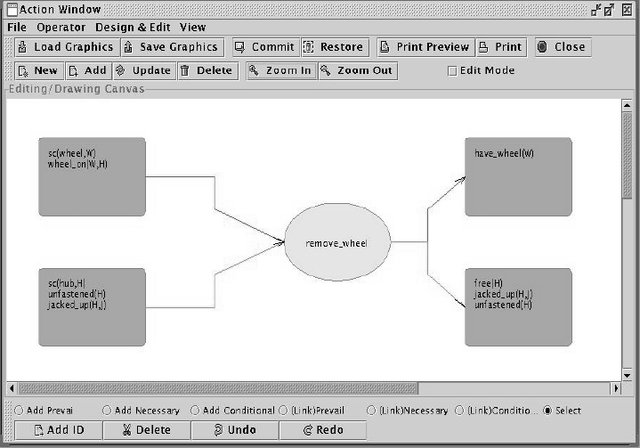
\includegraphics[width=0.7\linewidth]{figures/gipoaction}
	\caption{Screenshot of the operator editor tool in GIPO (\cite{mccluskey2005using})}
	\label{fig:gipoaction}
\end{figure}

\begin{figure}[h]
	\centering
	\includegraphics[width=0.7\linewidth]{figures/itsimple}
	\caption{Screenshot of a Planning UML model in itSIMPLE software (\cite{vaquero2013itsimple})}
	\label{fig:itSimple}
\end{figure}

\section{Discussions and Relations to Present Work}
Automated planning has found its application in a wide range of areas from virtual agent games (\cite{fernandez2006planning}) to space exploration (\cite{backes2004multi,bresina2005activity}).
A main research area has focused on integrating task planning with robot architectures \cite{cashmore2015rosplan}, in particular to handle time, resources and synchronisation (\cite{di2014planner,dvorak2014flexible}).
Combining task and motion planning is an open research problem and has been addressed previously (\cite{ferrer2015planning,garrett2015ffrob}), especially learning preconditions and effects of actions to be used in planning (\cite{ahmadzadeh2015learning,jetchev2013learning,konidaris2018fromSkills,ugur2015bottom}).
In these works, the focus often lies in grounding actions or learning symbolic action representations, so the robot is generally provided with a predefined set of motor skills that are refined by learning from plan traces or demonstrations.
%It is assumed that low-level actions have already been programmed and can be called directly after mapping them to PDDL actions.
For example, \citet{abdo2013learning} learns a fixed set of manipulation actions from user demonstrations, \ie stack blocks, pour from a bottle and open a door.
The robot only uses the actions to achieve a predefined task, \eg going through a door, but does not reuse them for unseen tasks.
%However, as the approach requires 5-10 demonstrations to learn action conditions, it becomes tedious and impractical if several actions need to be taught.

Automated planners can be very powerful for generating optimal plans for problems that even humans struggle to solve, \eg Tower of Hanoi problem (\cite{hanoiPddlGit}), Tetris (\cite{ipc14site}).
However, they are generally not accessible to end-users who do not have experience in this domain. 
While knowledge engineering tools facilitate the modelling of planning domains, they still require PDDL experts or common knowledge in software engineering.
In this thesis, we argue that end-users without this experience can still learn and use automated planning concepts to program robots.
We first conduct user studies (\chapt{chap:Pre-Experiments}) to evaluate this hypothesis and analyse the user's adoption when first presented to these concepts.
We then propose and implement a framework (\chapt{chap:Implementation}) that allows them to teach robots actions that can be used with an automated planner to solve previously unseen tasks.
We evaluate the implemented system and present experimental findings from a user study. %(\chapt{chap:Evaluation}).
%In general, the majority of tasks can be completed using the simple actions pick, move and drop. 
%For our framework, we considered planning problems, such as the Tower of Hanoi problem (\cite{douglas1985metamagical}) or a real-life game of Tetris (\cite{tetris}), which use these actions. 
%Since we focus on applications in cobotic environments, we wanted to choose a planning problem that occurs in real-world applications. 
%Therefore, we chose to evaluate the usability of our framework using the \texttt{PRODUCTION} planning domain, addressing the \texttt{PERMUTATION} planning problem. 
%It is then easy for the user to extrapolate from this simple example to any complex task.

%\fig{fig:planning-permutation} illustrates an example of the permutation planning problem. Given a description of the world state, \ie objects, types, properties (\fig{fig:planning-permutation}a,b), a set of possible atomic actions, and a goal state (\fig{fig:planning-permutation}d), the planner should generate the correct sequence of actions (\fig{fig:planning-permutation}c), which guarantees the transition from the initial world state to the goal state. Predicates are used to describe actions and object properties, such as \textit{``red cube is at position A"}: they can be \textit{instantiated} \texttt{(at redCube A)} or \textit{generalised} \texttt{(at ?cube ?posA)}, such that variables are prefixed with `?'.

%To allow a correct transition between different states of the world, actions are defined in terms of {preconditions} and {effects} (\fig{fig:action}). For a move action \texttt{(move cube A B)}, preconditions are the states required to perform the action  \texttt{(at cube A)}, and effects are the states obtained after the action \texttt{(at cube B)}. Classical planning algorithms use the Planning Domain Definition Language (PDDL) \cite{ghallab2004automated} as their standard encoding language, which extends the STRIPS \cite{fikes1971strips} formalism with greater expressivity, such as type structures (\fig{fig:planning-permutation}b). 

%Our proposed framework targets these domains and aims at solving related planning problems. It will allow the user to create action models and link the planning problem with the actual physical action executed by the robot.

% To Do: Discuss related work in terms of subjects that are addressed by Robot Programming by Demonstration in Cobotic Environments
